% Options for packages loaded elsewhere
\PassOptionsToPackage{unicode}{hyperref}
\PassOptionsToPackage{hyphens}{url}
%
\documentclass[
]{article}
\usepackage{amsmath,amssymb}
\usepackage{lmodern}
\usepackage{iftex}
\ifPDFTeX
  \usepackage[T1]{fontenc}
  \usepackage[utf8]{inputenc}
  \usepackage{textcomp} % provide euro and other symbols
\else % if luatex or xetex
  \usepackage{unicode-math}
  \defaultfontfeatures{Scale=MatchLowercase}
  \defaultfontfeatures[\rmfamily]{Ligatures=TeX,Scale=1}
\fi
% Use upquote if available, for straight quotes in verbatim environments
\IfFileExists{upquote.sty}{\usepackage{upquote}}{}
\IfFileExists{microtype.sty}{% use microtype if available
  \usepackage[]{microtype}
  \UseMicrotypeSet[protrusion]{basicmath} % disable protrusion for tt fonts
}{}
\makeatletter
\@ifundefined{KOMAClassName}{% if non-KOMA class
  \IfFileExists{parskip.sty}{%
    \usepackage{parskip}
  }{% else
    \setlength{\parindent}{0pt}
    \setlength{\parskip}{6pt plus 2pt minus 1pt}}
}{% if KOMA class
  \KOMAoptions{parskip=half}}
\makeatother
\usepackage{xcolor}
\IfFileExists{xurl.sty}{\usepackage{xurl}}{} % add URL line breaks if available
\IfFileExists{bookmark.sty}{\usepackage{bookmark}}{\usepackage{hyperref}}
\hypersetup{
  pdftitle={Homework 3},
  pdfauthor={Brandon Amaral, Monte Davityan, Nicholas Lombardo, Hongkai Lu},
  hidelinks,
  pdfcreator={LaTeX via pandoc}}
\urlstyle{same} % disable monospaced font for URLs
\usepackage[margin=1in]{geometry}
\usepackage{color}
\usepackage{fancyvrb}
\newcommand{\VerbBar}{|}
\newcommand{\VERB}{\Verb[commandchars=\\\{\}]}
\DefineVerbatimEnvironment{Highlighting}{Verbatim}{commandchars=\\\{\}}
% Add ',fontsize=\small' for more characters per line
\usepackage{framed}
\definecolor{shadecolor}{RGB}{248,248,248}
\newenvironment{Shaded}{\begin{snugshade}}{\end{snugshade}}
\newcommand{\AlertTok}[1]{\textcolor[rgb]{0.94,0.16,0.16}{#1}}
\newcommand{\AnnotationTok}[1]{\textcolor[rgb]{0.56,0.35,0.01}{\textbf{\textit{#1}}}}
\newcommand{\AttributeTok}[1]{\textcolor[rgb]{0.77,0.63,0.00}{#1}}
\newcommand{\BaseNTok}[1]{\textcolor[rgb]{0.00,0.00,0.81}{#1}}
\newcommand{\BuiltInTok}[1]{#1}
\newcommand{\CharTok}[1]{\textcolor[rgb]{0.31,0.60,0.02}{#1}}
\newcommand{\CommentTok}[1]{\textcolor[rgb]{0.56,0.35,0.01}{\textit{#1}}}
\newcommand{\CommentVarTok}[1]{\textcolor[rgb]{0.56,0.35,0.01}{\textbf{\textit{#1}}}}
\newcommand{\ConstantTok}[1]{\textcolor[rgb]{0.00,0.00,0.00}{#1}}
\newcommand{\ControlFlowTok}[1]{\textcolor[rgb]{0.13,0.29,0.53}{\textbf{#1}}}
\newcommand{\DataTypeTok}[1]{\textcolor[rgb]{0.13,0.29,0.53}{#1}}
\newcommand{\DecValTok}[1]{\textcolor[rgb]{0.00,0.00,0.81}{#1}}
\newcommand{\DocumentationTok}[1]{\textcolor[rgb]{0.56,0.35,0.01}{\textbf{\textit{#1}}}}
\newcommand{\ErrorTok}[1]{\textcolor[rgb]{0.64,0.00,0.00}{\textbf{#1}}}
\newcommand{\ExtensionTok}[1]{#1}
\newcommand{\FloatTok}[1]{\textcolor[rgb]{0.00,0.00,0.81}{#1}}
\newcommand{\FunctionTok}[1]{\textcolor[rgb]{0.00,0.00,0.00}{#1}}
\newcommand{\ImportTok}[1]{#1}
\newcommand{\InformationTok}[1]{\textcolor[rgb]{0.56,0.35,0.01}{\textbf{\textit{#1}}}}
\newcommand{\KeywordTok}[1]{\textcolor[rgb]{0.13,0.29,0.53}{\textbf{#1}}}
\newcommand{\NormalTok}[1]{#1}
\newcommand{\OperatorTok}[1]{\textcolor[rgb]{0.81,0.36,0.00}{\textbf{#1}}}
\newcommand{\OtherTok}[1]{\textcolor[rgb]{0.56,0.35,0.01}{#1}}
\newcommand{\PreprocessorTok}[1]{\textcolor[rgb]{0.56,0.35,0.01}{\textit{#1}}}
\newcommand{\RegionMarkerTok}[1]{#1}
\newcommand{\SpecialCharTok}[1]{\textcolor[rgb]{0.00,0.00,0.00}{#1}}
\newcommand{\SpecialStringTok}[1]{\textcolor[rgb]{0.31,0.60,0.02}{#1}}
\newcommand{\StringTok}[1]{\textcolor[rgb]{0.31,0.60,0.02}{#1}}
\newcommand{\VariableTok}[1]{\textcolor[rgb]{0.00,0.00,0.00}{#1}}
\newcommand{\VerbatimStringTok}[1]{\textcolor[rgb]{0.31,0.60,0.02}{#1}}
\newcommand{\WarningTok}[1]{\textcolor[rgb]{0.56,0.35,0.01}{\textbf{\textit{#1}}}}
\usepackage{graphicx}
\makeatletter
\def\maxwidth{\ifdim\Gin@nat@width>\linewidth\linewidth\else\Gin@nat@width\fi}
\def\maxheight{\ifdim\Gin@nat@height>\textheight\textheight\else\Gin@nat@height\fi}
\makeatother
% Scale images if necessary, so that they will not overflow the page
% margins by default, and it is still possible to overwrite the defaults
% using explicit options in \includegraphics[width, height, ...]{}
\setkeys{Gin}{width=\maxwidth,height=\maxheight,keepaspectratio}
% Set default figure placement to htbp
\makeatletter
\def\fps@figure{htbp}
\makeatother
\setlength{\emergencystretch}{3em} % prevent overfull lines
\providecommand{\tightlist}{%
  \setlength{\itemsep}{0pt}\setlength{\parskip}{0pt}}
\setcounter{secnumdepth}{-\maxdimen} % remove section numbering
\ifLuaTeX
  \usepackage{selnolig}  % disable illegal ligatures
\fi

\title{Homework 3}
\author{Brandon Amaral, Monte Davityan, Nicholas Lombardo, Hongkai Lu}
\date{2022-09-16}

\begin{document}
\maketitle

\begin{Shaded}
\begin{Highlighting}[]
\FunctionTok{library}\NormalTok{(tidyverse)}
\FunctionTok{library}\NormalTok{(ggplot2)}
\FunctionTok{library}\NormalTok{(GGally)}
\NormalTok{fire }\OtherTok{\textless{}{-}} \FunctionTok{read.csv}\NormalTok{(}\StringTok{"data/forestfires.csv"}\NormalTok{)}
\end{Highlighting}
\end{Shaded}

\begin{Shaded}
\begin{Highlighting}[]
\FunctionTok{head}\NormalTok{(fire)}
\end{Highlighting}
\end{Shaded}

\begin{verbatim}
##   X Y month day FFMC  DMC    DC  ISI temp RH wind rain area
## 1 7 5   mar fri 86.2 26.2  94.3  5.1  8.2 51  6.7  0.0    0
## 2 7 4   oct tue 90.6 35.4 669.1  6.7 18.0 33  0.9  0.0    0
## 3 7 4   oct sat 90.6 43.7 686.9  6.7 14.6 33  1.3  0.0    0
## 4 8 6   mar fri 91.7 33.3  77.5  9.0  8.3 97  4.0  0.2    0
## 5 8 6   mar sun 89.3 51.3 102.2  9.6 11.4 99  1.8  0.0    0
## 6 8 6   aug sun 92.3 85.3 488.0 14.7 22.2 29  5.4  0.0    0
\end{verbatim}

\begin{Shaded}
\begin{Highlighting}[]
\FunctionTok{str}\NormalTok{(fire)}
\end{Highlighting}
\end{Shaded}

\begin{verbatim}
## 'data.frame':    517 obs. of  13 variables:
##  $ X    : int  7 7 7 8 8 8 8 8 8 7 ...
##  $ Y    : int  5 4 4 6 6 6 6 6 6 5 ...
##  $ month: chr  "mar" "oct" "oct" "mar" ...
##  $ day  : chr  "fri" "tue" "sat" "fri" ...
##  $ FFMC : num  86.2 90.6 90.6 91.7 89.3 92.3 92.3 91.5 91 92.5 ...
##  $ DMC  : num  26.2 35.4 43.7 33.3 51.3 ...
##  $ DC   : num  94.3 669.1 686.9 77.5 102.2 ...
##  $ ISI  : num  5.1 6.7 6.7 9 9.6 14.7 8.5 10.7 7 7.1 ...
##  $ temp : num  8.2 18 14.6 8.3 11.4 22.2 24.1 8 13.1 22.8 ...
##  $ RH   : int  51 33 33 97 99 29 27 86 63 40 ...
##  $ wind : num  6.7 0.9 1.3 4 1.8 5.4 3.1 2.2 5.4 4 ...
##  $ rain : num  0 0 0 0.2 0 0 0 0 0 0 ...
##  $ area : num  0 0 0 0 0 0 0 0 0 0 ...
\end{verbatim}

\begin{Shaded}
\begin{Highlighting}[]
\FunctionTok{summary}\NormalTok{(fire)}
\end{Highlighting}
\end{Shaded}

\begin{verbatim}
##        X               Y          month               day           
##  Min.   :1.000   Min.   :2.0   Length:517         Length:517        
##  1st Qu.:3.000   1st Qu.:4.0   Class :character   Class :character  
##  Median :4.000   Median :4.0   Mode  :character   Mode  :character  
##  Mean   :4.669   Mean   :4.3                                        
##  3rd Qu.:7.000   3rd Qu.:5.0                                        
##  Max.   :9.000   Max.   :9.0                                        
##       FFMC            DMC              DC             ISI        
##  Min.   :18.70   Min.   :  1.1   Min.   :  7.9   Min.   : 0.000  
##  1st Qu.:90.20   1st Qu.: 68.6   1st Qu.:437.7   1st Qu.: 6.500  
##  Median :91.60   Median :108.3   Median :664.2   Median : 8.400  
##  Mean   :90.64   Mean   :110.9   Mean   :547.9   Mean   : 9.022  
##  3rd Qu.:92.90   3rd Qu.:142.4   3rd Qu.:713.9   3rd Qu.:10.800  
##  Max.   :96.20   Max.   :291.3   Max.   :860.6   Max.   :56.100  
##       temp             RH              wind            rain        
##  Min.   : 2.20   Min.   : 15.00   Min.   :0.400   Min.   :0.00000  
##  1st Qu.:15.50   1st Qu.: 33.00   1st Qu.:2.700   1st Qu.:0.00000  
##  Median :19.30   Median : 42.00   Median :4.000   Median :0.00000  
##  Mean   :18.89   Mean   : 44.29   Mean   :4.018   Mean   :0.02166  
##  3rd Qu.:22.80   3rd Qu.: 53.00   3rd Qu.:4.900   3rd Qu.:0.00000  
##  Max.   :33.30   Max.   :100.00   Max.   :9.400   Max.   :6.40000  
##       area        
##  Min.   :   0.00  
##  1st Qu.:   0.00  
##  Median :   0.52  
##  Mean   :  12.85  
##  3rd Qu.:   6.57  
##  Max.   :1090.84
\end{verbatim}

\begin{Shaded}
\begin{Highlighting}[]
\CommentTok{\#ggpairs(fire)}
\end{Highlighting}
\end{Shaded}

\begin{Shaded}
\begin{Highlighting}[]
\NormalTok{fire }\OtherTok{\textless{}{-}}\NormalTok{ fire }\SpecialCharTok{\%\textgreater{}\%} \FunctionTok{mutate}\NormalTok{(}\AttributeTok{month =} \FunctionTok{as.factor}\NormalTok{(month),}
                \AttributeTok{day =} \FunctionTok{as.factor}\NormalTok{(day))}
\end{Highlighting}
\end{Shaded}

\begin{Shaded}
\begin{Highlighting}[]
\CommentTok{\# Response area (multiple regression)}
\NormalTok{lm.fit }\OtherTok{\textless{}{-}} \FunctionTok{lm}\NormalTok{(area }\SpecialCharTok{\textasciitilde{}}\NormalTok{ ., }\AttributeTok{data =}\NormalTok{ fire )}
\FunctionTok{summary}\NormalTok{(lm.fit)}
\end{Highlighting}
\end{Shaded}

\begin{verbatim}
## 
## Call:
## lm(formula = area ~ ., data = fire)
## 
## Residuals:
##     Min      1Q  Median      3Q     Max 
##  -55.32  -17.84   -6.82    4.99 1039.28 
## 
## Coefficients:
##              Estimate Std. Error t value Pr(>|t|)  
## (Intercept) -15.16402   76.56086  -0.198   0.8431  
## X             2.25583    1.49786   1.506   0.1327  
## Y            -0.14765    2.81881  -0.052   0.9582  
## monthaug     46.88205   38.08792   1.231   0.2190  
## monthdec     47.37821   36.94830   1.282   0.2004  
## monthfeb      5.58985   25.94816   0.215   0.8295  
## monthjan     14.76909   56.40617   0.262   0.7936  
## monthjul     28.87889   33.05232   0.874   0.3827  
## monthjun      6.71548   30.33765   0.221   0.8249  
## monthmar     -4.22256   23.41447  -0.180   0.8570  
## monthmay     12.79646   50.91572   0.251   0.8017  
## monthnov     -4.41010   68.37767  -0.064   0.9486  
## monthoct     68.97536   45.42009   1.519   0.1295  
## monthsep     73.73192   42.67672   1.728   0.0847 .
## daymon        5.96928   10.48154   0.570   0.5693  
## daysat       19.40993   10.06218   1.929   0.0543 .
## daysun        5.14460    9.78870   0.526   0.5994  
## daythu        9.67192   11.10696   0.871   0.3843  
## daytue        7.79282   10.88291   0.716   0.4743  
## daywed        5.47914   11.40526   0.480   0.6312  
## FFMC         -0.09527    0.76985  -0.124   0.9016  
## DMC           0.20106    0.08681   2.316   0.0210 *
## DC           -0.12880    0.05872  -2.194   0.0287 *
## ISI          -0.54416    0.83105  -0.655   0.5129  
## temp          1.29620    1.03082   1.257   0.2092  
## RH           -0.13476    0.28845  -0.467   0.6406  
## wind          1.97427    1.77824   1.110   0.2674  
## rain         -2.81545    9.92647  -0.284   0.7768  
## ---
## Signif. codes:  0 '***' 0.001 '**' 0.01 '*' 0.05 '.' 0.1 ' ' 1
## 
## Residual standard error: 63.88 on 489 degrees of freedom
## Multiple R-squared:  0.04578,    Adjusted R-squared:  -0.006905 
## F-statistic: 0.8689 on 27 and 489 DF,  p-value: 0.6581
\end{verbatim}

\begin{Shaded}
\begin{Highlighting}[]
\FunctionTok{par}\NormalTok{(}\AttributeTok{mfrow=}\FunctionTok{c}\NormalTok{(}\DecValTok{2}\NormalTok{,}\DecValTok{2}\NormalTok{))}
\FunctionTok{plot}\NormalTok{(lm.fit)}
\end{Highlighting}
\end{Shaded}

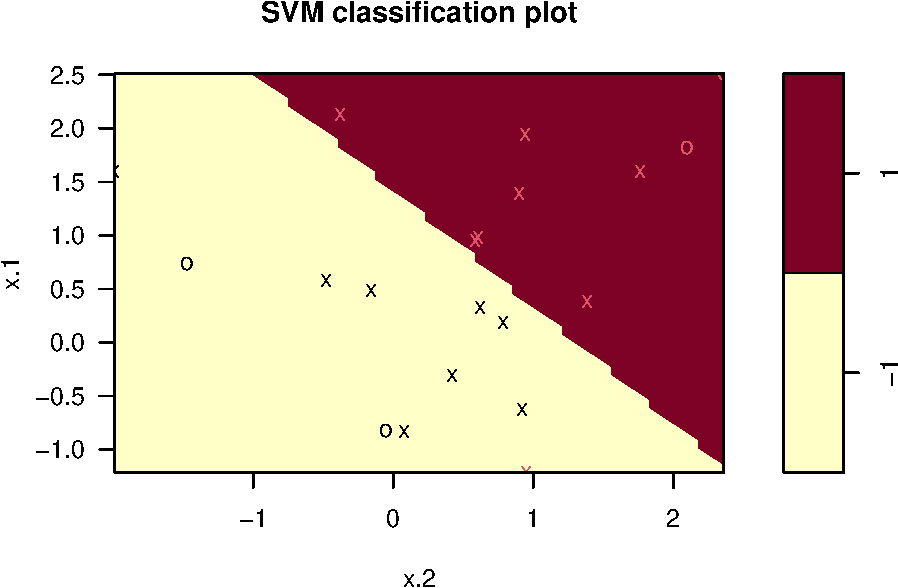
\includegraphics{Homework3_files/figure-latex/unnamed-chunk-6-1.pdf}

\begin{Shaded}
\begin{Highlighting}[]
\CommentTok{\# Response area (multiple regression) (Transformed Model)}
\NormalTok{lm.fit.transformed }\OtherTok{\textless{}{-}} \FunctionTok{lm}\NormalTok{(}\FunctionTok{log}\NormalTok{(area }\SpecialCharTok{+} \DecValTok{1}\NormalTok{) }\SpecialCharTok{\textasciitilde{}}\NormalTok{ ., }\AttributeTok{data =}\NormalTok{ fire )}
\FunctionTok{summary}\NormalTok{(lm.fit.transformed)}
\end{Highlighting}
\end{Shaded}

\begin{verbatim}
## 
## Call:
## lm(formula = log(area + 1) ~ ., data = fire)
## 
## Residuals:
##     Min      1Q  Median      3Q     Max 
## -1.9966 -1.0302 -0.5003  0.8284  5.1608 
## 
## Coefficients:
##               Estimate Std. Error t value Pr(>|t|)   
## (Intercept) -0.5705460  1.6566550  -0.344  0.73070   
## X            0.0524204  0.0324114   1.617  0.10645   
## Y           -0.0184700  0.0609946  -0.303  0.76216   
## monthaug     0.3274391  0.8241619   0.397  0.69132   
## monthdec     2.2050797  0.7995023   2.758  0.00603 **
## monthfeb     0.1886078  0.5614767   0.336  0.73708   
## monthjan    -0.3163816  1.2205397  -0.259  0.79558   
## monthjul     0.0991694  0.7151995   0.139  0.88978   
## monthjun    -0.2862231  0.6564584  -0.436  0.66302   
## monthmar    -0.3416243  0.5066518  -0.674  0.50045   
## monthmay     0.7175267  1.1017352   0.651  0.51518   
## monthnov    -1.1031443  1.4795838  -0.746  0.45628   
## monthoct     0.8232625  0.9828184   0.838  0.40263   
## monthsep     0.9934196  0.9234562   1.076  0.28256   
## daymon       0.1457734  0.2268038   0.643  0.52070   
## daysat       0.3099153  0.2177296   1.423  0.15526   
## daysun       0.2109897  0.2118118   0.996  0.31969   
## daythu       0.0722394  0.2403369   0.301  0.76387   
## daytue       0.3222933  0.2354888   1.369  0.17175   
## daywed       0.1978808  0.2467916   0.802  0.42305   
## FFMC         0.0074547  0.0166582   0.448  0.65471   
## DMC          0.0041790  0.0018785   2.225  0.02656 * 
## DC          -0.0020052  0.0012706  -1.578  0.11516   
## ISI         -0.0147970  0.0179825  -0.823  0.41099   
## temp         0.0360374  0.0223054   1.616  0.10682   
## RH           0.0006673  0.0062416   0.107  0.91490   
## wind         0.0603127  0.0384782   1.567  0.11766   
## rain         0.0309440  0.2147931   0.144  0.88551   
## ---
## Signif. codes:  0 '***' 0.001 '**' 0.01 '*' 0.05 '.' 0.1 ' ' 1
## 
## Residual standard error: 1.382 on 489 degrees of freedom
## Multiple R-squared:  0.07426,    Adjusted R-squared:  0.02315 
## F-statistic: 1.453 on 27 and 489 DF,  p-value: 0.06765
\end{verbatim}

\begin{Shaded}
\begin{Highlighting}[]
\FunctionTok{par}\NormalTok{(}\AttributeTok{mfrow=}\FunctionTok{c}\NormalTok{(}\DecValTok{2}\NormalTok{,}\DecValTok{2}\NormalTok{))}
\FunctionTok{plot}\NormalTok{(lm.fit.transformed)}
\end{Highlighting}
\end{Shaded}

\includegraphics{Homework3_files/figure-latex/unnamed-chunk-6-2.pdf}

\begin{Shaded}
\begin{Highlighting}[]
\CommentTok{\# Predict using LM for rows 15{-}25 and report MSE:}

\NormalTok{pred }\OtherTok{\textless{}{-}} \FunctionTok{predict}\NormalTok{(lm.fit, }\AttributeTok{newdata =}\NormalTok{ fire[}\DecValTok{15}\SpecialCharTok{:}\DecValTok{25}\NormalTok{,])}
\NormalTok{pred.transformed }\OtherTok{\textless{}{-}} \FunctionTok{predict}\NormalTok{(lm.fit.transformed, }\AttributeTok{newdata =}\NormalTok{ fire[}\DecValTok{15}\SpecialCharTok{:}\DecValTok{25}\NormalTok{,])}

\NormalTok{actual }\OtherTok{\textless{}{-}}\NormalTok{ fire[}\DecValTok{15}\SpecialCharTok{:}\DecValTok{25}\NormalTok{,] }\SpecialCharTok{\%\textgreater{}\%} \FunctionTok{select}\NormalTok{(area)}

\NormalTok{MSE }\OtherTok{\textless{}{-}} \FunctionTok{mean}\NormalTok{(}\FunctionTok{unlist}\NormalTok{((pred }\SpecialCharTok{{-}}\NormalTok{ actual)}\SpecialCharTok{\^{}}\DecValTok{2}\NormalTok{))}
\NormalTok{MSE}
\end{Highlighting}
\end{Shaded}

\begin{verbatim}
## [1] 611.4183
\end{verbatim}

\begin{Shaded}
\begin{Highlighting}[]
\NormalTok{MSE.transformed }\OtherTok{\textless{}{-}} \FunctionTok{mean}\NormalTok{(}\FunctionTok{unlist}\NormalTok{((pred.transformed }\SpecialCharTok{{-}}\NormalTok{ actual)}\SpecialCharTok{\^{}}\DecValTok{2}\NormalTok{))}
\NormalTok{MSE.transformed}
\end{Highlighting}
\end{Shaded}

\begin{verbatim}
## [1] 1.573042
\end{verbatim}

\begin{Shaded}
\begin{Highlighting}[]
\FunctionTok{plot}\NormalTok{(pred, }\FunctionTok{unlist}\NormalTok{(actual))}
\end{Highlighting}
\end{Shaded}

\includegraphics{Homework3_files/figure-latex/unnamed-chunk-7-1.pdf}

\begin{Shaded}
\begin{Highlighting}[]
\FunctionTok{plot}\NormalTok{(pred.transformed, }\FunctionTok{unlist}\NormalTok{(actual))}
\end{Highlighting}
\end{Shaded}

\includegraphics{Homework3_files/figure-latex/unnamed-chunk-7-2.pdf}

\begin{Shaded}
\begin{Highlighting}[]
\CommentTok{\# Binary area}
\NormalTok{fire }\OtherTok{\textless{}{-}}\NormalTok{ fire }\SpecialCharTok{\%\textgreater{}\%} 
  \FunctionTok{mutate}\NormalTok{(}\AttributeTok{binary\_area =} \FunctionTok{if\_else}\NormalTok{(area }\SpecialCharTok{!=} \DecValTok{0}\NormalTok{, }\StringTok{"Not zero"}\NormalTok{, }\StringTok{"Zero"}\NormalTok{)) }\SpecialCharTok{\%\textgreater{}\%} 
  \FunctionTok{mutate}\NormalTok{(}\AttributeTok{binary\_area =} \FunctionTok{as.factor}\NormalTok{(binary\_area))}

\NormalTok{glm.fit }\OtherTok{\textless{}{-}} \FunctionTok{glm}\NormalTok{(binary\_area }\SpecialCharTok{\textasciitilde{}}\NormalTok{ ., }\AttributeTok{family =} \StringTok{"binomial"}\NormalTok{, }\AttributeTok{data =}\NormalTok{ fire }\SpecialCharTok{\%\textgreater{}\%} \FunctionTok{select}\NormalTok{(}\SpecialCharTok{{-}}\NormalTok{area))}
\FunctionTok{summary}\NormalTok{(glm.fit)}
\end{Highlighting}
\end{Shaded}

\begin{verbatim}
## 
## Call:
## glm(formula = binary_area ~ ., family = "binomial", data = fire %>% 
##     select(-area))
## 
## Deviance Residuals: 
##     Min       1Q   Median       3Q      Max  
## -1.5873  -1.0993  -0.8112   1.1860   1.6016  
## 
## Coefficients:
##               Estimate Std. Error z value Pr(>|z|)
## (Intercept)  4.644e+00  2.888e+00   1.608    0.108
## X           -5.838e-02  4.806e-02  -1.215    0.225
## Y           -4.134e-02  9.078e-02  -0.455    0.649
## monthaug     2.074e-01  1.214e+00   0.171    0.864
## monthdec    -1.682e+01  7.894e+02  -0.021    0.983
## monthfeb    -4.220e-01  8.237e-01  -0.512    0.608
## monthjan     1.505e+01  1.556e+03   0.010    0.992
## monthjul     1.292e-01  1.054e+00   0.123    0.902
## monthjun     3.762e-01  9.718e-01   0.387    0.699
## monthmar     4.897e-01  7.494e-01   0.653    0.513
## monthmay    -8.583e-03  1.603e+00  -0.005    0.996
## monthnov     1.631e+01  2.400e+03   0.007    0.995
## monthoct     1.005e+00  1.456e+00   0.691    0.490
## monthsep    -5.052e-03  1.360e+00  -0.004    0.997
## daymon      -1.331e-01  3.400e-01  -0.391    0.695
## daysat      -6.636e-02  3.229e-01  -0.206    0.837
## daysun       1.264e-02  3.146e-01   0.040    0.968
## daythu       3.645e-03  3.569e-01   0.010    0.992
## daytue      -2.725e-01  3.504e-01  -0.778    0.437
## daywed      -3.474e-01  3.696e-01  -0.940    0.347
## FFMC        -3.146e-02  3.039e-02  -1.035    0.301
## DMC          1.138e-03  2.769e-03   0.411    0.681
## DC          -4.078e-04  1.871e-03  -0.218    0.827
## ISI          1.591e-02  2.803e-02   0.568    0.570
## temp        -4.861e-02  3.352e-02  -1.450    0.147
## RH          -5.851e-03  9.514e-03  -0.615    0.539
## wind        -8.036e-02  5.786e-02  -1.389    0.165
## rain        -6.886e-03  3.492e-01  -0.020    0.984
## 
## (Dispersion parameter for binomial family taken to be 1)
## 
##     Null deviance: 715.69  on 516  degrees of freedom
## Residual deviance: 678.24  on 489  degrees of freedom
## AIC: 734.24
## 
## Number of Fisher Scoring iterations: 15
\end{verbatim}

\begin{Shaded}
\begin{Highlighting}[]
\FunctionTok{set.seed}\NormalTok{(}\DecValTok{123}\NormalTok{)}

\NormalTok{training\_ind }\OtherTok{\textless{}{-}} \FunctionTok{sample}\NormalTok{(}\DecValTok{1}\SpecialCharTok{:}\DecValTok{517}\NormalTok{, }\FunctionTok{floor}\NormalTok{(.}\DecValTok{8}\SpecialCharTok{*}\DecValTok{517}\NormalTok{), }\AttributeTok{replace =} \ConstantTok{FALSE}\NormalTok{)}

\NormalTok{train }\OtherTok{\textless{}{-}}\NormalTok{ fire[training\_ind, }\FunctionTok{c}\NormalTok{(}\StringTok{"temp"}\NormalTok{,}\StringTok{"RH"}\NormalTok{,}\StringTok{"wind"}\NormalTok{,}\StringTok{"rain"}\NormalTok{, }\StringTok{"area"}\NormalTok{)]}
\NormalTok{val }\OtherTok{\textless{}{-}}\NormalTok{ fire[}\SpecialCharTok{{-}}\NormalTok{training\_ind, }\FunctionTok{c}\NormalTok{(}\StringTok{"temp"}\NormalTok{,}\StringTok{"RH"}\NormalTok{,}\StringTok{"wind"}\NormalTok{,}\StringTok{"rain"}\NormalTok{, }\StringTok{"area"}\NormalTok{)]}

\NormalTok{model.combos }\OtherTok{\textless{}{-}} \ControlFlowTok{function}\NormalTok{(model, }
\NormalTok{                         response, }
\NormalTok{                         predictors, }
\NormalTok{                         training, }
\NormalTok{                         validation, }
                         \AttributeTok{null.model =} \ConstantTok{TRUE}\NormalTok{,}
                         \AttributeTok{debug =} \ConstantTok{FALSE}\NormalTok{) \{}
  \StringTok{"This function iterates through all possible combos (2\^{}n){-}1 of }
\StringTok{    predictor variables and outputs the model with the best validation }
\StringTok{    MSE}
\StringTok{  }
\StringTok{    Inputs:}
\StringTok{      {-} model: A supervised regression learning model object (ie. lm)}
\StringTok{          Expecting the function to have formula and data parameters}
\StringTok{      {-} response: A string. The name of the response variable}
\StringTok{      {-} predictors: A vector of strings. The list of names of the     }
\StringTok{          predictor variables}
\StringTok{      {-} training: A data frame. The training set}
\StringTok{      {-} validation: A data frame. The validation set}
\StringTok{      {-} null.model: A boolean. (Optional). If TRUE, will compare the initial best}
\StringTok{          model as the null model (which is just the average). If set to FALSE,}
\StringTok{          the intial best model will be null and only the (2\^{}n){-}1 combos will be           considered}
\StringTok{      {-} debug: A boolean. (Optional). If TRUE print out the best.MSE and }
\StringTok{          best.predictions as they are being calculated}
\StringTok{      }
\StringTok{    Output:}
\StringTok{      {-} best.predictors: A list. Containing the names of the best }
\StringTok{        predictors (as measured by lowest validation MSE)}
\StringTok{      {-} best.mse: A number. The best MSE among the models}
\StringTok{  "}
  \CommentTok{\# Combinations is made from this code: }
  \CommentTok{\# https://stackoverflow.com/questions/40049313/generate{-}all{-}combinations{-}of{-}all{-}lengths{-}in{-}r{-}from{-}a{-}vector}
  \CommentTok{\# It generates the combinations of predictors as a list of strings}
\NormalTok{  combinations }\OtherTok{\textless{}{-}} \FunctionTok{do.call}\NormalTok{(}\StringTok{"c"}\NormalTok{, }\FunctionTok{lapply}\NormalTok{(}\FunctionTok{seq\_along}\NormalTok{(predictors), }\ControlFlowTok{function}\NormalTok{(i) }\FunctionTok{combn}\NormalTok{(predictors, i, }\AttributeTok{FUN =}\NormalTok{ list)))}
  
  \ControlFlowTok{if}\NormalTok{ (debug) \{}
    \FunctionTok{print}\NormalTok{(combinations)}
\NormalTok{  \}}
  
  \CommentTok{\# The validation response}
\NormalTok{  actual }\OtherTok{\textless{}{-}}\NormalTok{ validation[[response]]}
  
  \CommentTok{\# If null.model is TRUE, compare to the null model (the average)}
  \ControlFlowTok{if}\NormalTok{ (null.model) \{}
\NormalTok{    average.model }\OtherTok{\textless{}{-}} \FunctionTok{mean}\NormalTok{(training[[response]])}
\NormalTok{    best.MSE }\OtherTok{\textless{}{-}} \FunctionTok{mean}\NormalTok{((average.model }\SpecialCharTok{{-}}\NormalTok{ actual)}\SpecialCharTok{\^{}}\DecValTok{2}\NormalTok{)}
\NormalTok{    best.predictions }\OtherTok{\textless{}{-}} \FunctionTok{c}\NormalTok{(}\StringTok{"null model"}\NormalTok{)}
    
    \ControlFlowTok{if}\NormalTok{ (debug) \{}
      \FunctionTok{print}\NormalTok{(best.MSE)}
      \FunctionTok{print}\NormalTok{(}\StringTok{"null"}\NormalTok{)}
\NormalTok{    \}}
\NormalTok{  \}}
  \CommentTok{\# If null.model is FALSE, compare only the (2\^{}n){-}1 models}
  \ControlFlowTok{else}\NormalTok{ \{}
\NormalTok{    best.MSE }\OtherTok{\textless{}{-}} \ConstantTok{NA}
\NormalTok{    best.predictions }\OtherTok{\textless{}{-}} \ConstantTok{NA}
\NormalTok{  \}}
  
  
  \CommentTok{\# Loop through the combinations}
  \ControlFlowTok{for}\NormalTok{ (combo }\ControlFlowTok{in}\NormalTok{ combinations) \{}
    \CommentTok{\# Make the formula from the combos and the response}
\NormalTok{    formula }\OtherTok{\textless{}{-}} \FunctionTok{reformulate}\NormalTok{(combo, }\AttributeTok{response =}\NormalTok{ response)}
    \CommentTok{\# Fit the model using the given model and training data}
\NormalTok{    model.fit }\OtherTok{\textless{}{-}} \FunctionTok{model}\NormalTok{(}\AttributeTok{formula =}\NormalTok{ formula, }\AttributeTok{data =}\NormalTok{ training)}
    \CommentTok{\# Make predictions on the validation set}
\NormalTok{    preds }\OtherTok{\textless{}{-}} \FunctionTok{predict}\NormalTok{(model.fit, }\AttributeTok{newdata =}\NormalTok{ validation)}
    \CommentTok{\# Calculate validation MSE using the predictions}
\NormalTok{    MSE.validation }\OtherTok{\textless{}{-}} \FunctionTok{mean}\NormalTok{(}\FunctionTok{unlist}\NormalTok{((preds }\SpecialCharTok{{-}}\NormalTok{ actual)}\SpecialCharTok{\^{}}\DecValTok{2}\NormalTok{))}
    \CommentTok{\# Update the best.predictions if the MSE is lower then the prior }
      \CommentTok{\# best}
    \ControlFlowTok{if}\NormalTok{ (debug) \{}
      \FunctionTok{print}\NormalTok{(MSE.validation)}
      \FunctionTok{print}\NormalTok{(combo)}
\NormalTok{    \}}
    
    \ControlFlowTok{if}\NormalTok{ (}\FunctionTok{is.na}\NormalTok{(best.MSE) }\SpecialCharTok{||}\NormalTok{ MSE.validation }\SpecialCharTok{\textless{}}\NormalTok{ best.MSE) \{}
\NormalTok{      best.MSE }\OtherTok{\textless{}{-}}\NormalTok{ MSE.validation}
\NormalTok{      best.predictions }\OtherTok{\textless{}{-}}\NormalTok{ combo}
\NormalTok{    \}}
\NormalTok{  \}}
  
  \CommentTok{\# Return best.MSE and best.predictions}
  \FunctionTok{return}\NormalTok{(}\FunctionTok{list}\NormalTok{(}\AttributeTok{Best.MSE =}\NormalTok{ best.MSE, }\AttributeTok{Best.Combination =}\NormalTok{ best.predictions))}
\NormalTok{\}}

\FunctionTok{model.combos}\NormalTok{(lm, }\StringTok{"area"}\NormalTok{, }\FunctionTok{c}\NormalTok{(}\StringTok{"temp"}\NormalTok{,}\StringTok{"RH"}\NormalTok{,}\StringTok{"wind"}\NormalTok{,}\StringTok{"rain"}\NormalTok{), train, val, }\ConstantTok{TRUE}\NormalTok{, }\ConstantTok{FALSE}\NormalTok{)}
\end{Highlighting}
\end{Shaded}

\begin{verbatim}
## $Best.MSE
## [1] 972.3262
## 
## $Best.Combination
## [1] "wind"
\end{verbatim}

\begin{Shaded}
\begin{Highlighting}[]
\CommentTok{\#lm(y \textasciitilde{} x1 + x2)}
\CommentTok{\#lm(y \textasciitilde{} x1 + x4 + x3)}
\CommentTok{\#lm(y \textasciitilde{} x1 + x2 + x3 + x4)}
\end{Highlighting}
\end{Shaded}

\hypertarget{chapter-3-summary}{%
\section{Chapter 3 Summary:}\label{chapter-3-summary}}

\hypertarget{section-3.1}{%
\subsection{Section 3.1:}\label{section-3.1}}

\hypertarget{section-3.2}{%
\subsection{Section 3.2:}\label{section-3.2}}

\hypertarget{section-3.3}{%
\subsection{Section 3.3:}\label{section-3.3}}

\hypertarget{section-3.4}{%
\subsection{Section 3.4:}\label{section-3.4}}

Exploring the relationship between sales and advertising budget: Since
there are three variables that make up advertising budget (TV, radio,
and newspaper), a multiple linear regression model is used with TV,
radio and newspaper as the predictors and sales as the response. An
F-statistic can be used to test if
\(H_0: \beta_{TV} = \beta_{radio} = \beta_{newspaper} = 0\). For this
dataset, the pvalue was low providing significant evidence of the
relationship between sales and advertising budget.

Strenght of the relationship:RSE which estimates the standard deviation
of the response (in this case the sales) between the population
regression line; and, \(R^2\) which is the percentage of variability of
the response explained by the predictors are two good measures for the
strength of a relationship between response and predictors.

Which media are association with sales?: Individual pvalues of the
predictors can be viewed to identify the significance of any individual
predictor to the response.

How large is the association between each medium and sales?:
Constructing confidence intervals for the individual \(\hat{\beta}\)
coefficients is a good way to go about measure the size of association
between the predictors and the response. If the confidence interval
includes 0, then it may suggest a predictor has non- significant impact
on the response. However, collinearity could be an issue which results
in large confidence bounds. VIF scores can be viewed to ensure
collinearity is not an issue. Another technique to identify individual
relationships between the predictors and response is to perform simple
linear regression models between each predictor and response and
identify size of association.

How accurately can we predict future sales?: If we are interested in an
individual response then we can use a prediction interval, but if
interested in an average response we can use a confidence interval. The
bounds for prediction intervals are always wider then confidence
intervals due to taking into account irreducible error.

Is the relationship linear?: A residual diagnostic plot can be used to
identify linearity. We expect no pattern (centered at 0) among the
residuals if the relationship is linear. Transformations can be used if
patterns are found.

Is there synergy among the advertising media?:Interactions among
variables should be explored.

\hypertarget{section-3.5-comparison-of-linear-regression-with-k-nearest-neighbors}{%
\subsection{Section 3.5: Comparison of Linear Regression with K-Nearest
Neighbors}\label{section-3.5-comparison-of-linear-regression-with-k-nearest-neighbors}}

Linear regression is a parametric method due to its linearity
assumption. The advantage to parametric methods is they are easy to fit
because of the small number of parameters to estimate, tests for
significance are easy to perform, and interpretation is usually clear.
The disadvantage of parametric methods are their strong assumptions. If
the true model deviates from our assumed model, then the results will be
poor.

Non- parametric methods do not have assumptions of the model form and
are generally more flexible then parametric methods.

\hypertarget{knn-regression}{%
\subsubsection{KNN Regression:}\label{knn-regression}}

Is very similar to KNN classifier (but for when the response is
continuous) in that the model will identify the K closest points to a
point of prediction (denoted as \(N_0\)) and averages those to form the
prediction.

\[\hat{f}(x_0) = \frac{1}{K}\sum_{x_i \in N_0} y_i\] The best value of K
is based on the bias- variance trade off. Smaller K will have lower bias
but higher variance whereas larger values of K will have higher bias but
lower variance. KNN can suffer from the curse of dimensionality where in
higher dimensions, the K observations closest to the point of prediction
may be very off.

In the choice between parametric or non- parametric methods, if the true
form of the relationship matches the parametric models assumptions, then
it will outperform the non- parametric method.

``In general, parametric methods will tend to outperform non- parametric
approaches when there is a small number of observations per predictor''.

\end{document}
